% Chapitre 18 -- Z-GWAYA : un portail « fermé par défaut » pour le code écrit par des modèles de langage (v3, v3.1)
% Sources : results/discovery_journal_2026/TOP20.json (pick 18) ; zenodo_inventory.json (23119953, 23120120) ;
% rapport gwaya_v3_verified_report.pdf et results/gwaya_v3_oracle_eval.json du dépôt Zenodo 23119953 (lus, non exécutés) ;
% README du dépôt public GWAYA-GwenLayaOpenModel (gh api, 26/10/2026).
% Rejeu local de la démonstration 1 = 2 : code/fig18.py. Figure : code/fig18.py.
\chapter[Une porte fermée par défaut]{Une porte qui reste fermée quand on ne sait pas}
\reference{Publié le 3 octobre 2026. Version 3~: doi:10.5281/zenodo.23119953~; version 3.1~: doi:10.5281/zenodo.23120120.}

\noindent\niveau{C} pour la sûreté du portail~: c'est un raisonnement, mené par des agents d'IA sous la direction de
l'auteur, et mesuré seulement sur un petit corpus écrit par le projet lui-même. La démonstration \og $1=2$\fg{} est un fait que chacun peut refaire~; nous l'avons
refaite.

\section*{L'idée en une image}

\begin{analogie}
Imaginez une porte qui ne s'ouvre que si chaque gardien a signé~: celui qui vérifie que la valise n'est pas vide,
celui qui vérifie l'orthographe des papiers, celui qui vérifie les tampons. Si un gardien est absent, la porte
reste fermée~: on ne remplace pas une signature manquante par un \og sans doute\fg. C'est ce qu'on appelle
\og fermé par défaut\fg.

\emph{Où l'image cesse d'être juste~:} les gardiens contrôlent la \emph{forme} des papiers, pas les intentions du
voyageur. Un programme bien écrit qui fait autre chose que ce qu'on voulait passe la porte.
\end{analogie}

\section*{Ce qui a été fait}

Les modèles de langage écrivent du code qui a l'air juste. Parfois il est vide, rempli de bouche-trous, mal typé, ou,
pour une preuve, \og démontré\fg{} par une échappatoire. GWAYA est un filtre placé entre le modèle et l'utilisateur.
Sa version~3 n'accepte un programme que si de vrais outils disent oui~: un audit qui repère les bouche-trous
(\texttt{pass}, \texttt{...}, les noms en \texttt{mock\_}), l'analyseur de Python, le vérificateur de types du langage
Rust, et, pour une preuve, le noyau de Lean suivi d'un audit des axiomes. Quand un outil manque, la réponse est
\og non vérifié\fg, jamais \og accepté\fg. Avant cette version, un compilateur absent valait\ldots{} une réussite.

\paragraph{Un exemple à suivre au crayon.} Voici trois lignes de Lean.
\begin{center}
\texttt{def s : String := "-{}-" axiom bad : False}\\
\texttt{theorem t : 1 = 2 := bad.elim}
\end{center}
La première ligne déclare un texte qui vaut \texttt{"-{}-"}, puis, en cachette, un \emph{axiome}~: une affirmation
admise sans preuve, ici \og le faux est vrai\fg. La deuxième en déduit $1=2$. Un filtre qui lit le texte et efface
les commentaires voit \texttt{-{}-}, croit que la suite de la ligne est un commentaire, et ne voit pas l'axiome.
Lean, lui, compile le fichier sans une erreur~: le code de sortie vaut~$0$, celui d'un succès. Seule la commande
qui demande au noyau la liste des axiomes utilisés trahit la ruse~:
\texttt{\textquotesingle t\textquotesingle{} depends on axioms: [bad]}. Le 26 octobre 2026, nous avons relancé ces lignes sur la machine du projet,
avec une version plus récente de Lean~: code de sortie $0$, et exactement cette ligne. Un vérificateur qui se fie au
seul code de sortie aurait certifié que $1=2$.

\section*{Comment on s'est assuré que ce n'est pas faux}

Le rapport ne publie que ce que des tests du dépôt soutiennent. L'auteur a écrit 26 cas, chacun avec la réponse
attendue, et les a passés chacun 5 fois au portail (figure~\ref{fig:c18}). Sur les 24 cas que le portail est censé
traiter, aucune erreur~: 8 bons programmes acceptés, 16 mauvais refusés, et des verdicts identiques à chaque
passage. Deux cas étaient là pour échouer~: un programme qui soustrait au lieu d'additionner, en Python et en Rust.
Le portail les a acceptés tous les deux, comme prévu, puisqu'il juge la forme et non le sens. Un autre cas, une
preuve correcte dont un commentaire contenait le mot \og axiom\fg, avait d'abord été refusé à tort~; le défaut a été
corrigé, et le rapport précise que ce cas ne compte donc plus comme une preuve indépendante.

Le rapport retire aussi des chiffres des versions précédentes~: une comparaison \og 20 sur 20 contre 5 sur 20\fg{}
face à un modèle plus gros, faite avec des validateurs qui cherchaient un bout de texte~; une \og exactitude de
96~\%\fg~; des temps de démarrage. Le dépôt raconte ensuite une rétractation de plus~: une révision de la
version~3.1 annonçait un gain d'au moins 8 points sur la foi d'un fichier de résultats écrit à la main. Mesuré pour
de vrai, sur 257 problèmes, le gain a été de $7{,}78$ points~; le seuil de 8 avait été fixé à l'avance, et le
verdict est publié tel quel~: échec.

\section*{Ce que ça ne dit pas}

\begin{limite}
\begin{itemize}
\item 26 cas écrits par l'auteur ne mesurent pas un taux d'erreur sur du vrai code produit par des modèles~; zéro
  erreur sur ce corpus ne donne aucun intervalle de confiance digne de ce nom.
\item Les audits des chiffres du dépôt sont ceux de l'auteur. Personne d'autre n'a relu le travail.
\item Le portail vérifie la bonne forme, pas que le programme fait ce qu'on voulait, ni que l'énoncé d'un
  théorème dit ce qu'on croit.
\item La partie Lean traite un fichier isolé, sans la grande bibliothèque mathématique, et repère les déclarations
  par une recherche de motifs, pas avec l'analyseur de Lean.
\item Plus tard dans l'année, le projet a trouvé qu'on peut tromper même la liste des axiomes, par une option qui
  saute le contrôle du noyau~; seul un rejeu complet des preuves l'attrape.
\end{itemize}
\end{limite}

\section*{Pour aller plus loin}

Les deux versions et leur archive de reproduction (sources, tests, résultats bruts, empreintes de contrôle) sont
sous doi:10.5281/zenodo.23119953 et doi:10.5281/zenodo.23120120~; le dépôt public du projet les prolonge
(GWAYA-GwenLayaOpenModel). Le chapitre~\ref{ch:c19} montre la même leçon appliquée au banc d'essai du projet lui-même.

\begin{figure}[t]
\centering
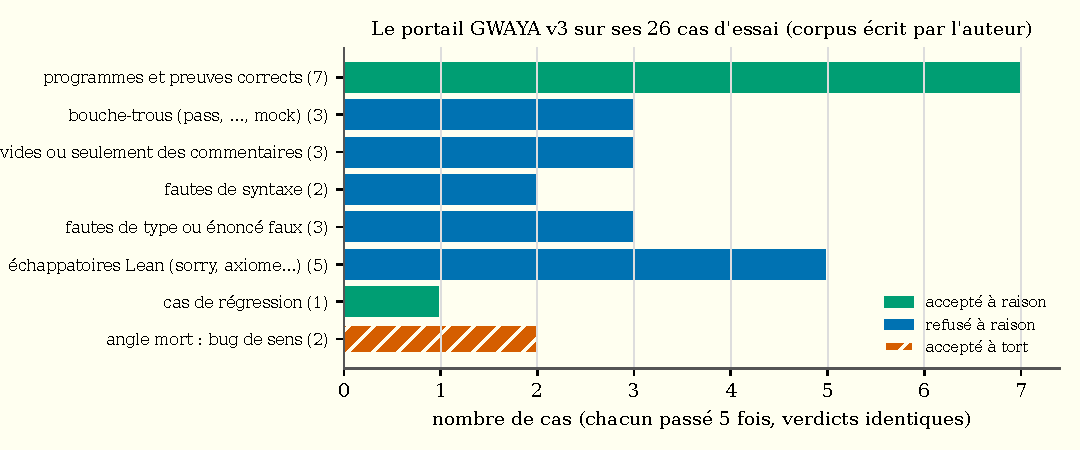
\includegraphics[width=\linewidth]{figures/c18_portail}
\caption{Les 26 cas d'essai de GWAYA~v3, comptés à partir du fichier de résultats publié. Tout est juste sauf les
deux angles morts prévus~: du code qui fait autre chose que voulu, accepté parce qu'il est bien formé.}
\label{fig:c18}
\end{figure}
